%%
%% Automatically generated file from DocOnce source
%% (https://github.com/hplgit/doconce/)
%%

% #define PREAMBLE

% #ifdef PREAMBLE
%-------------------- begin preamble ----------------------

\documentclass[%
oneside,                 % oneside: electronic viewing, twoside: printing
final,                   % draft: marks overfull hboxes, figures with paths
10pt]{article}

\listfiles               % print all files needed to compile this document

\usepackage{relsize,makeidx,color,setspace,amsmath,amsfonts,amssymb}
\usepackage[table]{xcolor}
\usepackage{bm,microtype}

\usepackage[pdftex]{graphicx}

% Packages for typesetting blocks of computer code
\usepackage{fancyvrb,framed,moreverb}

% Define colors
\definecolor{orange}{cmyk}{0,0.4,0.8,0.2}
\definecolor{tucorange}{rgb}{1.0,0.64,0}
\definecolor{darkorange}{rgb}{.71,0.21,0.01}
\definecolor{darkgreen}{rgb}{.12,.54,.11}
\definecolor{myteal}{rgb}{.26, .44, .56}
\definecolor{gray}{gray}{0.45}
\definecolor{mediumgray}{gray}{.8}
\definecolor{lightgray}{gray}{.95}
\definecolor{brown}{rgb}{0.54,0.27,0.07}
\definecolor{purple}{rgb}{0.5,0.0,0.5}
\definecolor{darkgray}{gray}{0.25}
\definecolor{darkblue}{rgb}{0,0.08,0.45}
\definecolor{darkblue2}{rgb}{0,0,0.8}
\definecolor{lightred}{rgb}{1.0,0.39,0.28}
\definecolor{lightgreen}{rgb}{0.48,0.99,0.0}
\definecolor{lightblue}{rgb}{0.53,0.81,0.92}
\definecolor{lightblue2}{rgb}{0.3,0.3,1.0}
\definecolor{lightpurple}{rgb}{0.87,0.63,0.87}
\definecolor{lightcyan}{rgb}{0.5,1.0,0.83}

\colorlet{comment_green}{green!50!black}
\colorlet{string_red}{red!60!black}
\colorlet{keyword_pink}{magenta!70!black}
\colorlet{indendifier_green}{green!70!white}

% Backgrounds for code
\definecolor{cbg_gray}{rgb}{.95, .95, .95}
\definecolor{bar_gray}{rgb}{.92, .92, .92}

\definecolor{cbg_yellowgray}{rgb}{.95, .95, .85}
\definecolor{bar_yellowgray}{rgb}{.95, .95, .65}

\colorlet{cbg_yellow2}{yellow!10}
\colorlet{bar_yellow2}{yellow!20}

\definecolor{cbg_yellow1}{rgb}{.98, .98, 0.8}
\definecolor{bar_yellow1}{rgb}{.98, .98, 0.4}

\definecolor{cbg_red1}{rgb}{1, 0.85, 0.85}
\definecolor{bar_red1}{rgb}{1, 0.75, 0.85}

\definecolor{cbg_blue1}{rgb}{0.87843, 0.95686, 1.0}
\definecolor{bar_blue1}{rgb}{0.7,     0.95686, 1}

%\setlength{\fboxsep}{-1.5mm}  % adjust cod_vpad/pro_vpad background box

%% Background for code blocks (parameter is color name)

%% pro/cod_vpad: gives some vertical padding before and after the text
%% (but has more simplistic code than _cod/pro_tight+cod/pro).
%% pro/cod_vpad can be used to enclose Verbatim or lst begin/end for code.
%% pro/cod calls _pro/cod_tight and has very little vertical padding,
%% used to enclose Verbatim and other begin/end for code.
%% (pro/cod is what the ptex2tex program could produce with the
%% Blue/BlueBar definitions in .ptex2tex.cfg.)

\newenvironment{cod_vpad}[1]{
   \def\FrameCommand{\colorbox{#1}}
   \MakeFramed{\FrameRestore}}
   {\endMakeFramed}

\newenvironment{_cod_tight}[1]{
   \def\FrameCommand{\colorbox{#1}}
   \FrameRule0.6pt\MakeFramed {\FrameRestore}\vskip3mm}
   {\vskip0mm\endMakeFramed}

\newenvironment{cod}[1]{
\bgroup\rmfamily
\fboxsep=0mm\relax
\begin{_cod_tight}{#1}
\list{}{\parsep=-2mm\parskip=0mm\topsep=0pt\leftmargin=2mm
\rightmargin=2\leftmargin\leftmargin=4pt\relax}
\item\relax}
{\endlist\end{_cod_tight}\egroup}

%% Background for complete program blocks (parameter 1 is color name
%% for background, parameter 2 is color for left bar)
\newenvironment{pro_vpad}[2]{
   \def\FrameCommand{\color{#2}\vrule width 1mm\normalcolor\colorbox{#1}}
   \MakeFramed{\FrameRestore}}
   {\endMakeFramed}

\newenvironment{_pro_tight}[2]{
   \def\FrameCommand{\color{#2}\vrule width 1mm\normalcolor\colorbox{#1}}
   \FrameRule0.6pt\MakeFramed {\advance\hsize-2mm\FrameRestore}\vskip3mm}
   {\vskip0mm\endMakeFramed}

\newenvironment{pro}[2]{
\bgroup\rmfamily
\fboxsep=0mm\relax
\begin{_pro_tight}{#1}{#2}
\list{}{\parsep=-2mm\parskip=0mm\topsep=0pt\leftmargin=2mm
\rightmargin=2\leftmargin\leftmargin=4pt\relax}
\item\relax}
{\endlist\end{_pro_tight}\egroup}

\usepackage{listingsutf8}

% Common lstlisting parameters
\lstset{
  basicstyle=\small \ttfamily,
  breaklines=false,          % break/wrap lines
  breakatwhitespace=true,    % let linebreaks happen at whitespace
  breakindent=40pt,
  tab=,
  tabsize=4,                 % tab means 4 spaces
  %belowskip=\smallskipamount,  % space between code and text below
  xleftmargin=5pt,           % indentation of code frame
  xrightmargin=5pt,
  framexleftmargin=5pt,      % add frame space to the left of code
  %numbers=left,             % put line numbers on the left
  %stepnumber=2,             % stepnumber=1 numbers each line, =n every n lines
  %framerule=0.4pt           % thickness of frame
  aboveskip=2ex,             % vertical space above code frame
  showstringspaces=false,    % show spaces in strings with an underscore
  showspaces=false,          % show spaces with an underscore
  showtabs=false,
  keepspaces=true,
  columns=fullflexible,      % tighter character kerning, like verb
  escapeinside={||},         % for |\pause| in slides and math in code blocks
  extendedchars=\true,       % allows non-ascii chars, does not work with utf-8
}

% Internally defined styles for lstlisting

\lstdefinestyle{simple}{
commentstyle={},
}

% end of custom lstdefinestyles

\usepackage[T1]{fontenc}
%\usepackage[latin1]{inputenc}
\usepackage{ucs}
\usepackage[utf8x]{inputenc}

\usepackage{lmodern}         % Latin Modern fonts derived from Computer Modern

% Hyperlinks in PDF:
\definecolor{linkcolor}{rgb}{0,0,0.4}
\usepackage{hyperref}
\hypersetup{
    breaklinks=true,
    colorlinks=true,
    linkcolor=linkcolor,
    urlcolor=linkcolor,
    citecolor=black,
    filecolor=black,
    %filecolor=blue,
    pdfmenubar=true,
    pdftoolbar=true,
    bookmarksdepth=3   % Uncomment (and tweak) for PDF bookmarks with more levels than the TOC
    }
%\hyperbaseurl{}   % hyperlinks are relative to this root

\setcounter{tocdepth}{2}  % number chapter, section, subsection

% Tricks for having figures close to where they are defined:
% 1. define less restrictive rules for where to put figures
\setcounter{topnumber}{2}
\setcounter{bottomnumber}{2}
\setcounter{totalnumber}{4}
\renewcommand{\topfraction}{0.95}
\renewcommand{\bottomfraction}{0.95}
\renewcommand{\textfraction}{0}
\renewcommand{\floatpagefraction}{0.75}
% floatpagefraction must always be less than topfraction!
% 2. ensure all figures are flushed before next section
\usepackage[section]{placeins}
% 3. enable begin{figure}[H] (often leads to ugly pagebreaks)
%\usepackage{float}\restylefloat{figure}

\usepackage[framemethod=TikZ]{mdframed}

% --- begin definitions of admonition environments ---

% --- end of definitions of admonition environments ---

% prevent orhpans and widows
\clubpenalty = 10000
\widowpenalty = 10000

% --- end of standard preamble for documents ---


% insert custom LaTeX commands...

\raggedbottom
\makeindex
\usepackage[totoc]{idxlayout}   % for index in the toc
\usepackage[nottoc]{tocbibind}  % for references/bibliography in the toc

%-------------------- end preamble ----------------------

\begin{document}

% matching end for #ifdef PREAMBLE
% #endif

\newcommand{\half}{\frac{1}{2}}
\newcommand{\halfi}{{1/2}}
\newcommand{\tp}{\thinspace .}

\newcommand{\uex}{{u_{\small\mbox{e}}}}
\newcommand{\uexd}[1]{{u_{\small\mbox{e}, #1}}}
\newcommand{\vex}{{v_{\small\mbox{e}}}}
\newcommand{\vexd}[1]{{v_{\small\mbox{e}, #1}}}
\newcommand{\Aex}{{A_{\small\mbox{e}}}}

% Operators
\newcommand{\Ddt}[1]{\frac{D #1}{dt}}
\newcommand{\E}[1]{\hbox{E}\lbrack #1 \rbrack}
\newcommand{\Var}[1]{\hbox{Var}\lbrack #1 \rbrack}
\newcommand{\Std}[1]{\hbox{Std}\lbrack #1 \rbrack}

\newcommand{\xpoint}{\bm{x}}
\newcommand{\normalvec}{\bm{n}}
\newcommand{\Oof}[1]{\mathcal{O}(#1)}

% Boldface vectors/tensors
\newcommand{\x}{\bm{x}}
\newcommand{\X}{\bm{X}}
\renewcommand{\u}{\bm{u}}
\renewcommand{\v}{\bm{v}}
\newcommand{\w}{\bm{w}}
\newcommand{\acc}{\bm{a}}
\newcommand{\rpos}{\bm{r}}
\newcommand{\V}{\bm{V}}
\newcommand{\e}{\bm{e}}
\newcommand{\f}{\bm{f}}
\newcommand{\F}{\bm{F}}
\newcommand{\stress}{\bm{\sigma}}
\newcommand{\strain}{\bm{\varepsilon}}
\newcommand{\stressc}{{\sigma}}
\newcommand{\strainc}{{\varepsilon}}
\newcommand{\I}{\bm{I}}
\newcommand{\T}{\bm{T}}

\newcommand{\dfc}{\alpha}  % diffusion coefficient
% Unit vectors
\newcommand{\ii}{\bm{i}}
\newcommand{\jj}{\bm{j}}
\newcommand{\kk}{\bm{k}}
\newcommand{\ir}{\bm{i}_r}
\newcommand{\ith}{\bm{i}_{\theta}}
\newcommand{\iz}{\bm{i}_z}

% Index sets
\newcommand{\Ix}{\mathcal{I}_x}
\newcommand{\Iy}{\mathcal{I}_y}
\newcommand{\Iz}{\mathcal{I}_z}
\newcommand{\It}{\mathcal{I}_t}
%\newcommand{\Ix}{{I_x}}
%\newcommand{\Iy}{{I_y}}
%\newcommand{\Iz}{{I_z}}
%\newcommand{\It}{{I_t}}
%\newcommand{\If}{\mathcal{I}}     % for FEM
\newcommand{\If}{\mathcal{I}_s}     % for FEM
%\newcommand{\If}{{I}}     % for FEM
%\newcommand{\Ifd}{\mathcal{I}_d}  % for FEM
\newcommand{\Ifd}{{I_d}}  % for FEM
\newcommand{\Ifb}{{I_b}}  % for FEM
\newcommand{\setb}[1]{#1^0}    % set begin
\newcommand{\sete}[1]{#1^{-1}} % set end
%\newcommand{\setl}[1]{#1\setminus\{\set1{#1}\}}
%\newcommand{\setr}[1]{#1\setminus\{\set0{#1}\}}
%\newcommand{\seti}[1]{#1\setminus\{\set0{#1},\set1{#1}\}}
\newcommand{\setl}[1]{#1^-}
\newcommand{\setr}[1]{#1^+}
\newcommand{\seti}[1]{#1^i}
\newcommand{\sequencei}[1]{\left\{ {#1}_i \right\}_{i\in\If}}

% Finite elements
\newcommand{\basphi}{\varphi}
\newcommand{\baspsi}{\psi}
\newcommand{\refphi}{\tilde\basphi}
\newcommand{\psib}{\bm{\psi}}
\newcommand{\sinL}[1]{\sin\left((#1+1)\pi\frac{x}{L}\right)}
\newcommand{\xno}[1]{x_{#1}}
%\newcommand{\xno}[1]{x^{(#1)}}
\newcommand{\Xno}[1]{X_{(#1)}}
\newcommand{\yno}[1]{y_{#1}}
\newcommand{\Yno}[1]{Y_{(#1)}}
\newcommand{\xdno}[1]{\bm{x}_{#1}}

% FEniCS commands
\newcommand{\dX}{\, \mathrm{d}X}
\newcommand{\dx}{\, \mathrm{d}x}
\newcommand{\ds}{\, \mathrm{d}s}
\newcommand{\Real}{\mathbb{R}}
\newcommand{\Integerp}{\mathbb{N}}
\newcommand{\Integer}{\mathbb{Z}}


% ------------------- main content ----------------------



% ----------------- title -------------------------

\thispagestyle{empty}

\begin{center}
{\LARGE\bf
\begin{spacing}{1.25}
Study guide: Analysis of exponential decay models
\end{spacing}
}
\end{center}

% ----------------- author(s) -------------------------

\begin{center}
{\bf Hans Petter Langtangen${}^{1, 2}$} \\ [0mm]
\end{center}

\begin{center}
% List of all institutions:
\centerline{{\small ${}^1$Center for Biomedical Computing, Simula Research Laboratory}}
\centerline{{\small ${}^2$Department of Informatics, University of Oslo}}
\end{center}
    
% ----------------- end author(s) -------------------------

% --- begin date ---
\begin{center}
Oct 10, 2015
\end{center}
% --- end date ---

\vspace{1cm}


% !split
\section*{Analysis of finite difference equations}
\label{decay:analysis}

Model:
\begin{equation}
u'(t) = -au(t),\quad u(0)=I
\end{equation}

Method:
\begin{equation}
u^{n+1} = \frac{1 - (1-\theta) a\Delta t}{1 + \theta a\Delta t}u^n
\label{decay:analysis:scheme}
\end{equation}


% --- begin paragraph admon ---
\paragraph{Problem setting.}
How good is this method? Is it safe to use it?
% --- end paragraph admon ---



% !split
\subsection*{Encouraging numerical solutions}

$I=1$, $a=2$, $\theta =1,0.5, 0$, $\Delta t=1.25, 0.75, 0.5, 0.1$.



% inline figure
\centerline{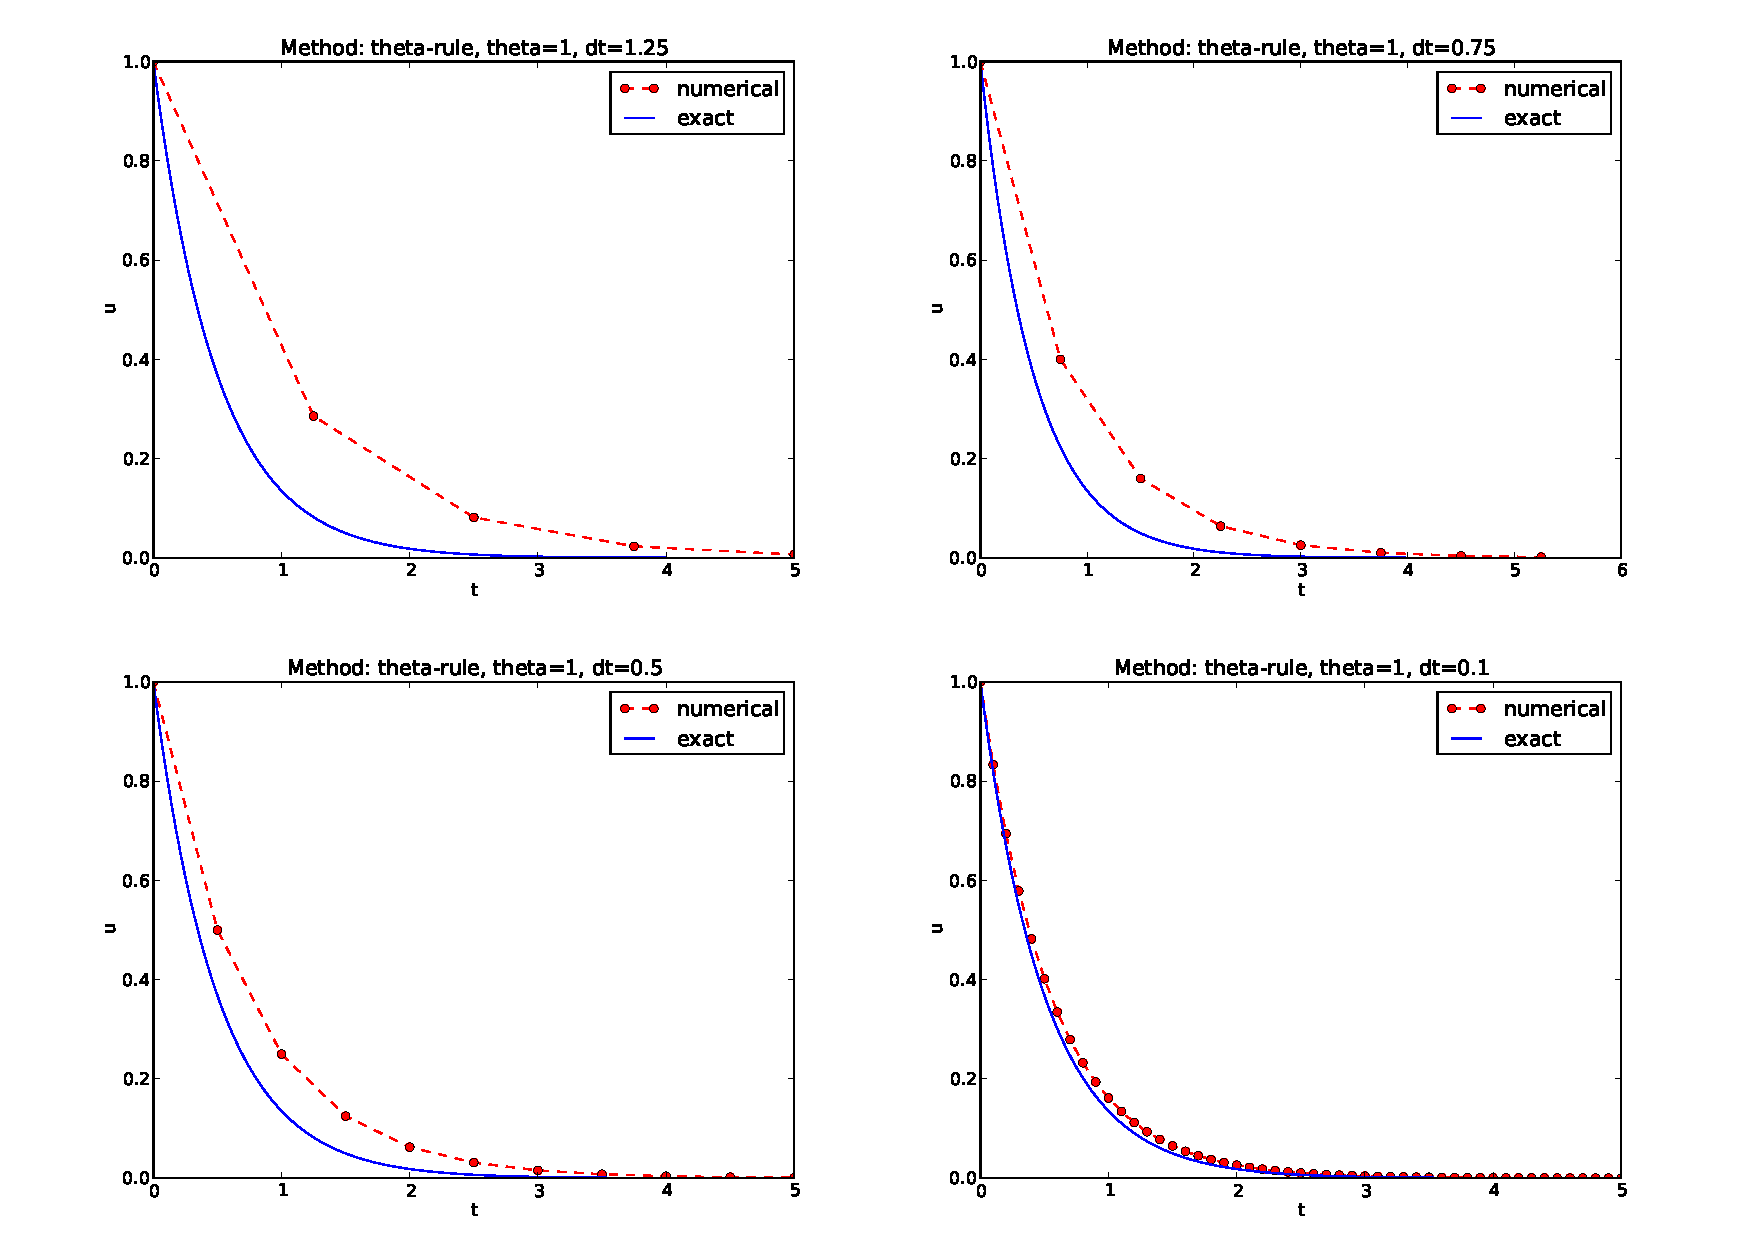
\includegraphics[width=1.1\linewidth]{fig-analysis/BE4c.pdf}}



% !split
\subsection*{Discouraging numerical solutions; Crank-Nicolson}



% inline figure
\centerline{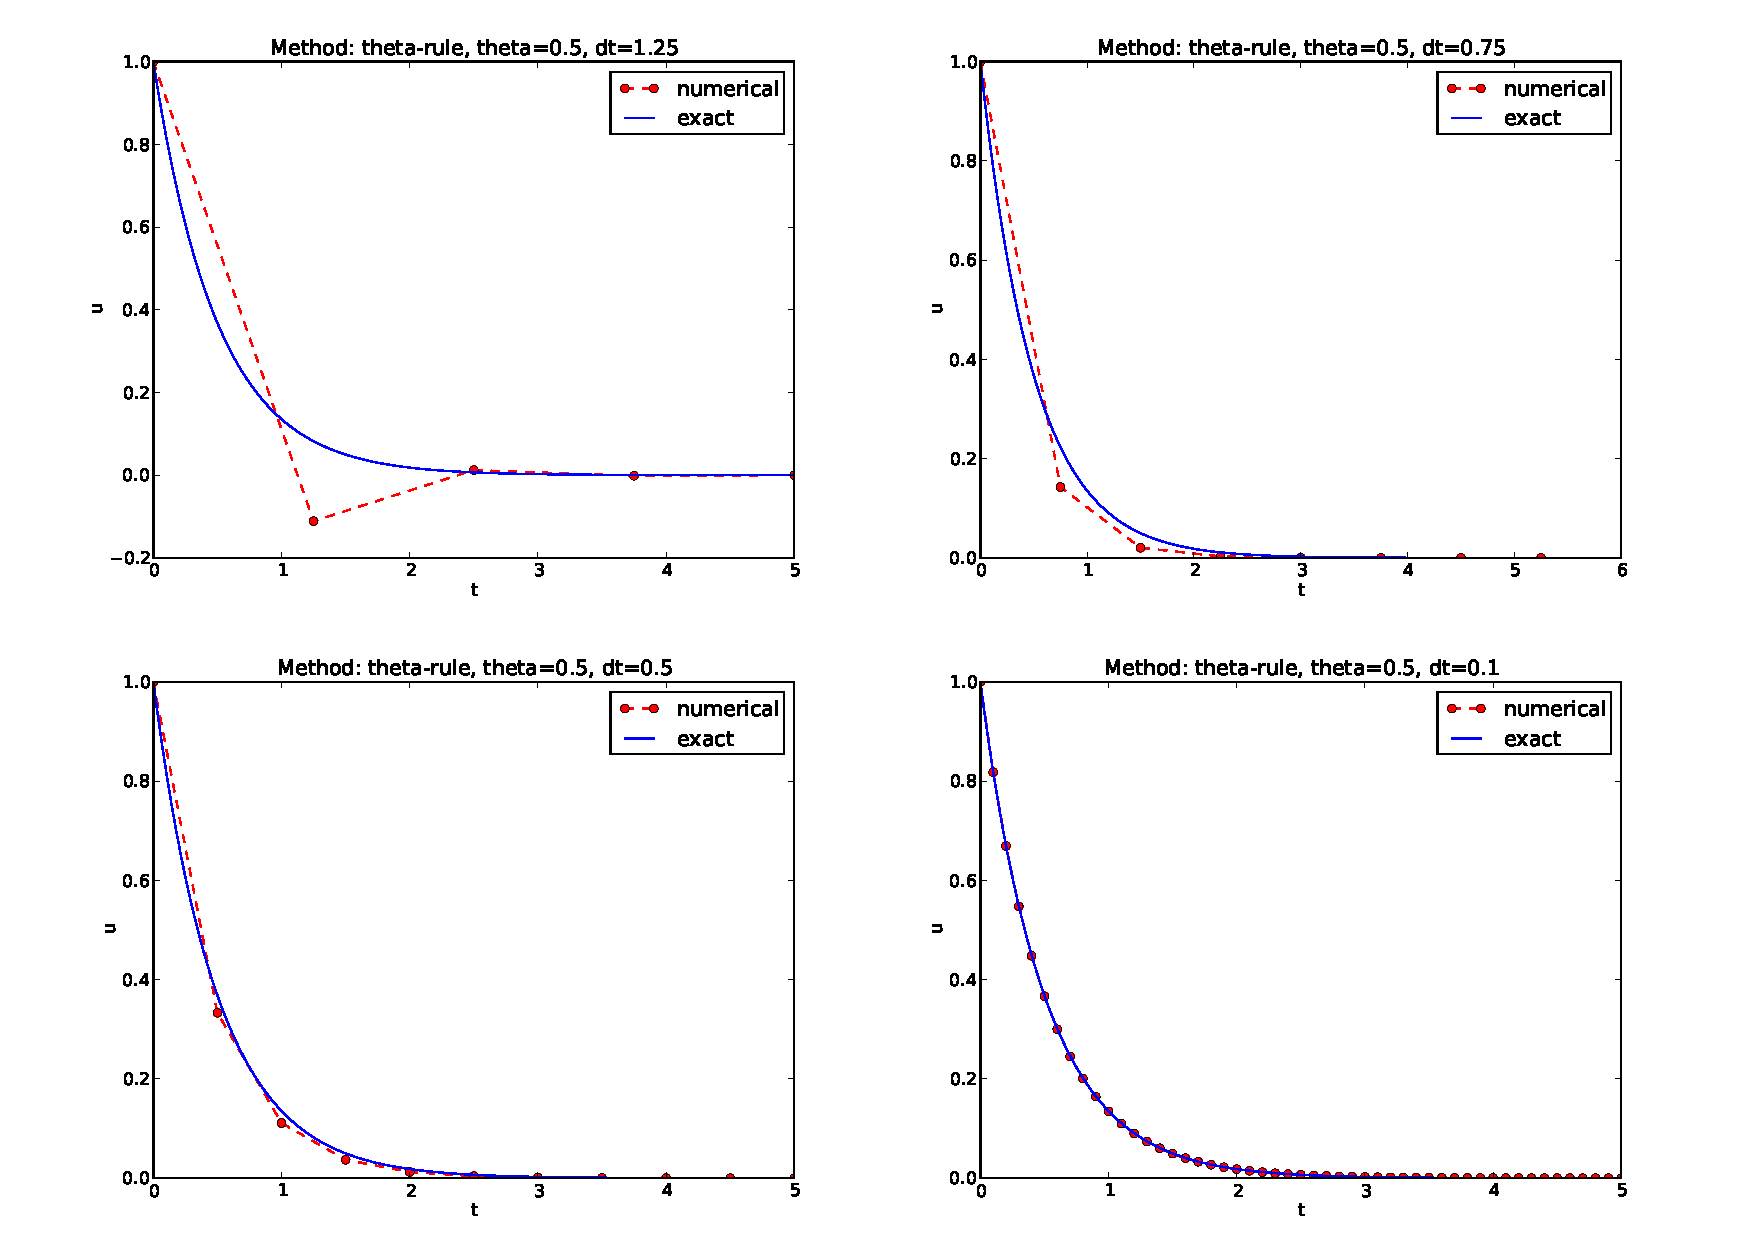
\includegraphics[width=1.1\linewidth]{fig-analysis/CN4c.pdf}}



% !split
\subsection*{Discouraging numerical solutions; Forward Euler}



% inline figure
\centerline{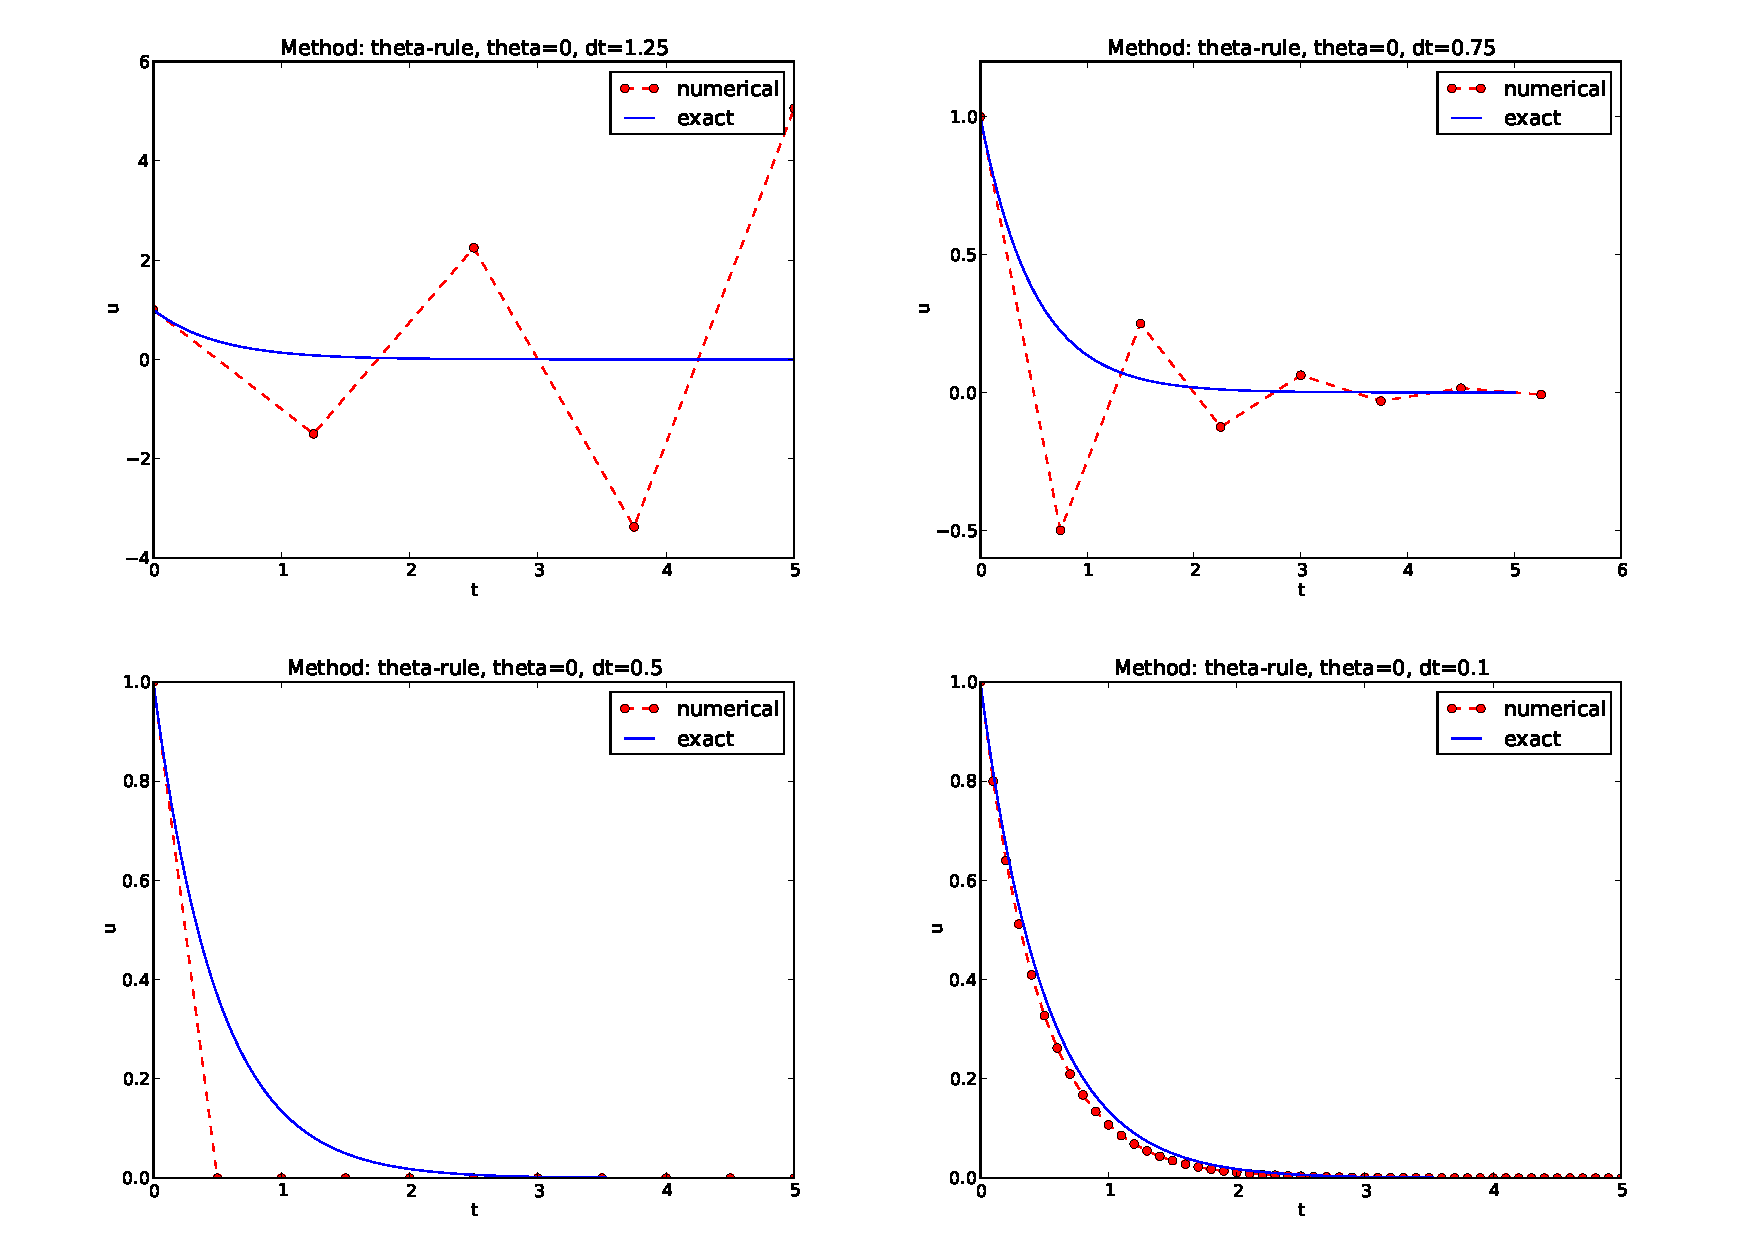
\includegraphics[width=1.1\linewidth]{fig-analysis/FE4c.pdf}}



% !split
\subsection*{Summary of observations}

The characteristics of the displayed curves can be summarized as follows:

\begin{itemize}
  \item The Backward Euler scheme \emph{always} gives a monotone solution, lying above
    the exact curve.

  \item The Crank-Nicolson scheme gives the most accurate results, but for
    $\Delta t=1.25$ the solution oscillates.

  \item The Forward Euler scheme gives a growing, oscillating solution for
    $\Delta t=1.25$; a decaying, oscillating solution for $\Delta t=0.75$;
    a strange solution $u^n=0$ for $n\geq 1$ when $\Delta t=0.5$; and
    a solution seemingly as accurate as the one by the Backward Euler
    scheme for $\Delta t = 0.1$, but the curve lies \emph{below} the exact
    solution.
\end{itemize}

\noindent
% !split
\subsection*{Problem setting}


% --- begin paragraph admon ---
\paragraph{Goal.}
We ask the question

\begin{itemize}
  \item Under what circumstances, i.e., values of
    the input data $I$, $a$, and $\Delta t$ will the Forward Euler and
    Crank-Nicolson schemes result in undesired oscillatory solutions?
\end{itemize}

\noindent
Techniques of investigation:

\begin{itemize}
 \item Numerical experiments

 \item Mathematical analysis
\end{itemize}

\noindent
Another question to be raised is

\begin{itemize}
 \item How does $\Delta t$ impact the error in the numerical solution?
\end{itemize}

\noindent
% --- end paragraph admon ---



% !split
\subsection*{Experimental investigation of oscillatory solutions}

The solution is oscillatory if
\[ u^{n} > u^{n-1}\]



% inline figure
\centerline{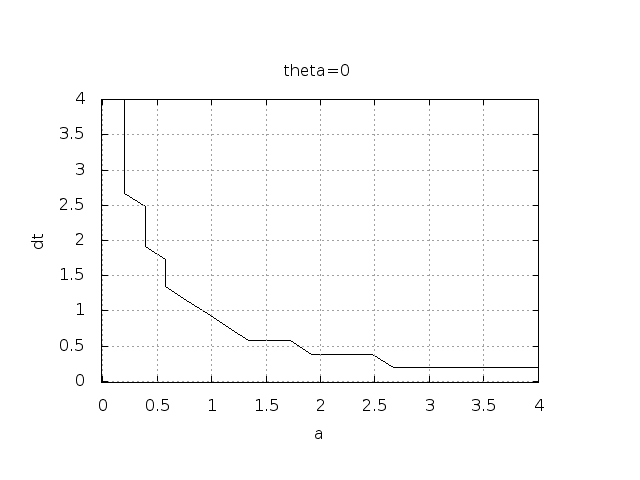
\includegraphics[width=0.9\linewidth]{fig-analysis/osc_region_FE.png}}



Seems that $a\Delta t < 1$ for FE and 2 for CN.

% !split
\subsection*{Exact numerical solution}

Starting with $u^0=I$, the simple recursion (\ref{decay:analysis:scheme})
can be applied repeatedly $n$ times, with the result that

\begin{equation}
u^{n} = IA^n,\quad A = \frac{1 - (1-\theta) a\Delta t}{1 + \theta a\Delta t}
\label{decay:analysis:unex}
\end{equation}

Such an exact discrete solution is unusual, but very handy for analysis.

% !split
\subsection*{Stability}

\index{stability}

Since $u^n\sim A^n$,

\begin{itemize}
 \item $A < 0$ gives a factor $(-1)^n$ and oscillatory solutions

 \item $|A|>1$ gives growing solutions

 \item Recall: the exact solution is \emph{monotone} and \emph{decaying}

 \item If these qualitative properties are not met, we say that the
   numerical solution is \emph{unstable}
\end{itemize}

\noindent
% !split
\subsection*{Computation of stability in this problem}

$A < 0$ if

\[
\frac{1 - (1-\theta) a\Delta t}{1 + \theta a\Delta t} < 0
\]
To avoid oscillatory solutions we must have $A> 0$ and

\begin{equation}
\Delta t < \frac{1}{(1-\theta)a}\ 
\end{equation}

\begin{itemize}
 \item Always fulfilled for Backward Euler

 \item $\Delta t \leq 1/a$ for Forward Euler

 \item $\Delta t \leq 2/a$ for Crank-Nicolson
\end{itemize}

\noindent
% !split
\subsection*{Computation of stability in this problem}

$|A|\leq 1$ means $-1\leq A\leq 1$

\begin{equation}
-1\leq\frac{1 - (1-\theta) a\Delta t}{1 + \theta a\Delta t} \leq 1
\label{decay:th:stability}
\end{equation}
$-1$ is the critical limit:

\begin{align*}
\Delta t &\leq \frac{2}{(1-2\theta)a},\quad \theta < \half\\ 
\Delta t &\geq \frac{2}{(1-2\theta)a},\quad \theta > {\half}
\end{align*}

\begin{itemize}
 \item Always fulfilled for Backward Euler and Crank-Nicolson

 \item $\Delta t \leq 2/a$ for Forward Euler
\end{itemize}

\noindent
% !split
\subsection*{Explanation of problems with Forward Euler}



% inline figure
\centerline{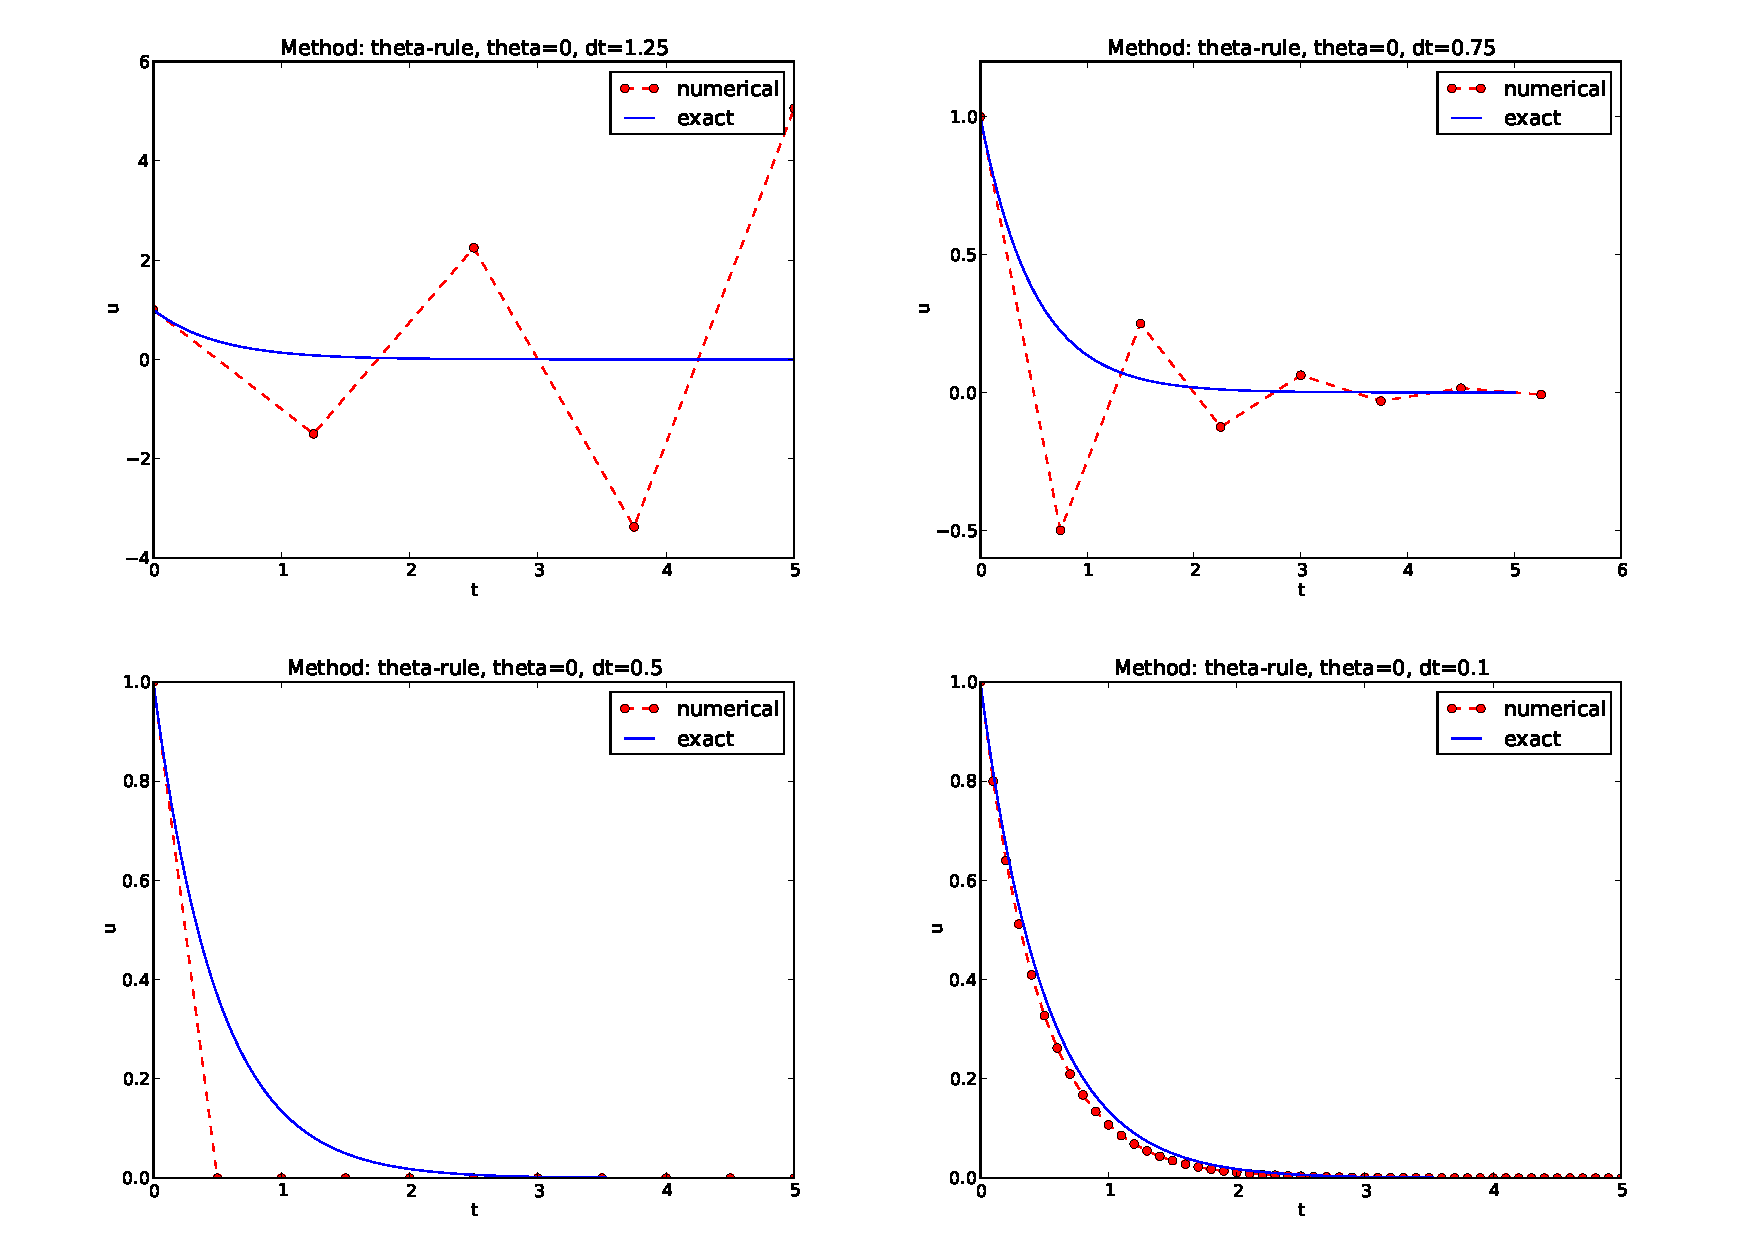
\includegraphics[width=1.1\linewidth]{fig-analysis/FE4c.pdf}}



\begin{itemize}
 \item $a\Delta t= 2\cdot 1.25=2.5$ and $A=-1.5$: oscillations and growth

 \item $a\Delta t = 2\cdot 0.75=1.5$ and $A=-0.5$: oscillations and decay

 \item $\Delta t=0.5$ and $A=0$: $u^n=0$ for $n>0$

 \item Smaller $Delta t$: qualitatively correct solution
\end{itemize}

\noindent
% !split
\subsection*{Explanation of problems with Crank-Nicolson}



% inline figure
\centerline{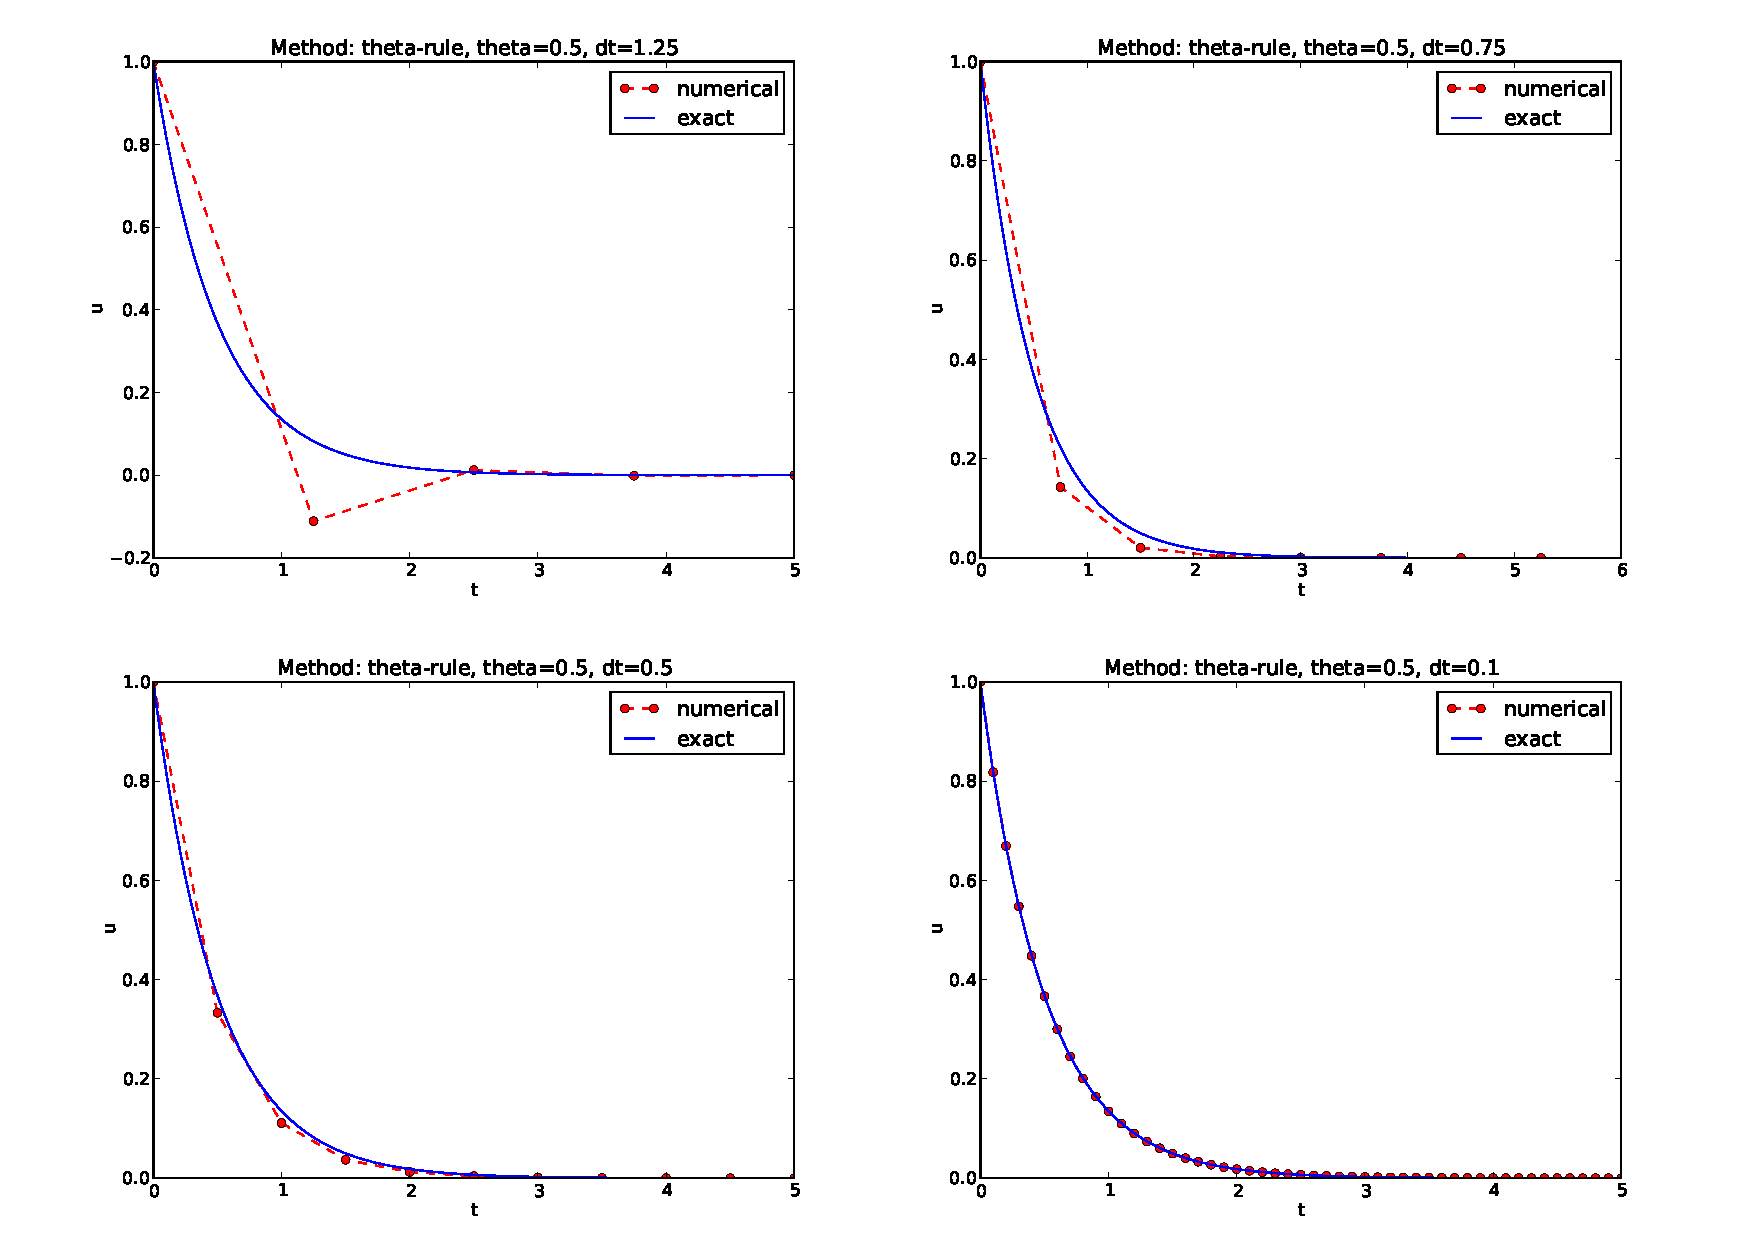
\includegraphics[width=1.1\linewidth]{fig-analysis/CN4c.pdf}}



\begin{itemize}
 \item $\Delta t=1.25$ and $A=-0.25$: oscillatory solution

 \item Never any growing solution
\end{itemize}

\noindent
% !split
\subsection*{Summary of stability}

\begin{enumerate}
\item Forward Euler is \emph{conditionally stable}
\begin{itemize}

   \item $\Delta t < 2/a$ for avoiding growth

   \item $\Delta t\leq 1/a$ for avoiding oscillations

\end{itemize}

\noindent
\item The Crank-Nicolson is \emph{unconditionally stable} wrt growth
   and conditionally stable wrt oscillations
\begin{itemize}

   \item $\Delta t < 2/a$ for avoiding oscillations

\end{itemize}

\noindent
\item Backward Euler is unconditionally stable
\end{enumerate}

\noindent
% !split
\subsection*{Comparing amplification factors}

$u^{n+1}$ is an amplification $A$ of $u^n$:

\[ u^{n+1} = Au^n,\quad A = \frac{1 - (1-\theta) a\Delta t}{1 + \theta a\Delta t} \]

The exact solution is also an amplification:

\[ u(t_{n+1}) = \Aex u(t_n), \quad \Aex = e^{-a\Delta t}\]

A possible measure of accuracy: $\Aex - A$

% !split
\subsection*{Plot of amplification factors}



% inline figure
\centerline{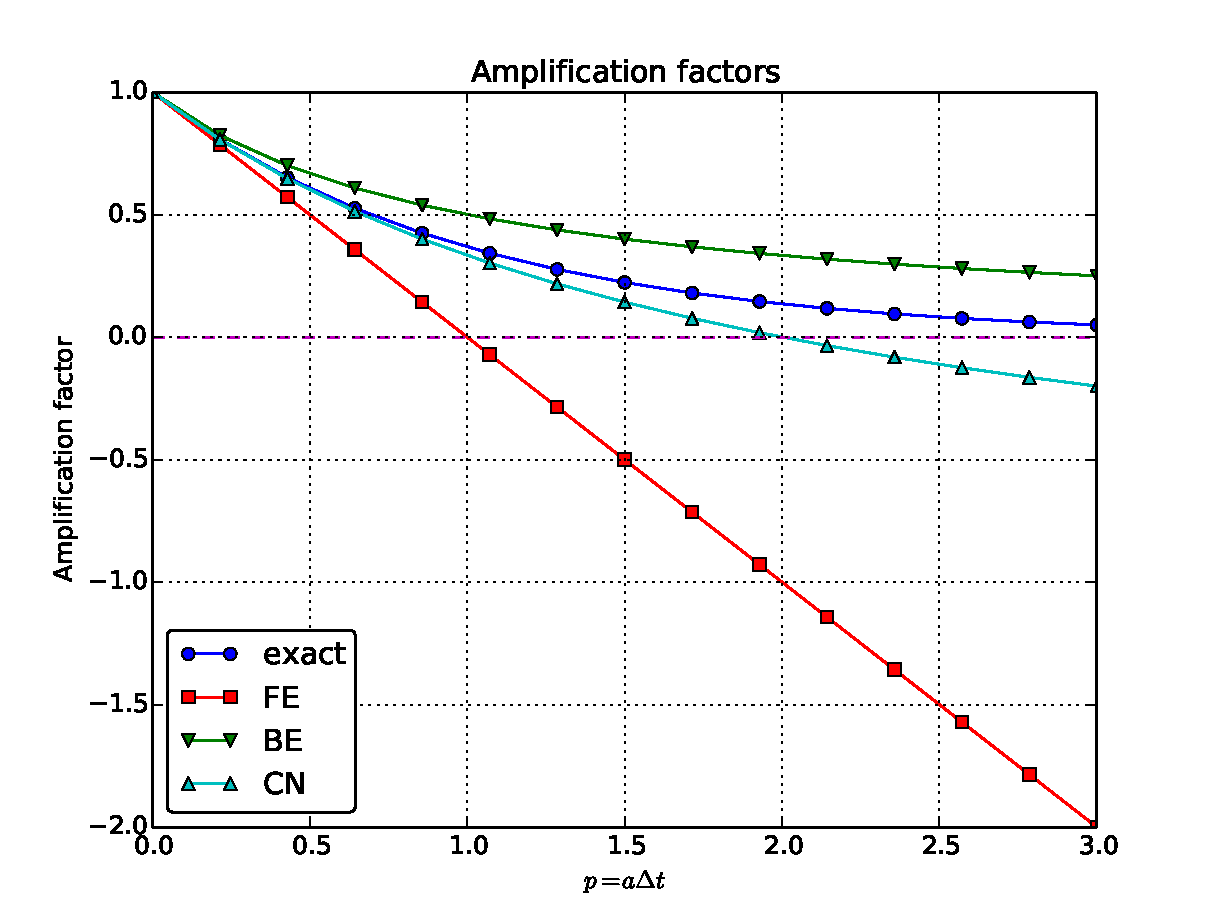
\includegraphics[width=0.9\linewidth]{fig-analysis/A_factors.pdf}}



% !split
\subsection*{$p=a\Delta t$ is the important parameter for numerical performance}

\begin{itemize}
 \item $p=a\Delta t$ is a dimensionless parameter

 \item all expressions for stability and accuracy involve $p$

 \item Note that $\Delta t$ alone is not so important, it is the
   combination with $a$ through $p=a\Delta t$ that matters
\end{itemize}

\noindent

% --- begin paragraph admon ---
\paragraph{Another ``proof'' why $p=a\Delta t$ is key.}
If we scale the model
by $\bar t=at$, $\bar u=u/I$, we get
$d\bar u/d\bar t = -\bar u$, $\bar u(0)=1$ (no physical parameters!).
The analysis show that $\Delta \bar t$ is key, corresponding to
$a\Delta t$ in the unscaled model.
% --- end paragraph admon ---



% !split
\subsection*{Series expansion of amplification factors}

To investigate $\Aex - A$ mathematically, we
can Taylor expand the expression, using $p=a\Delta t$ as variable.

\begin{cod}{cbg_yellow2}\begin{lstlisting}[language=Python,style=simple,xleftmargin=2mm]
>>> from sympy import *
>>> # Create p as a mathematical symbol with name 'p'
>>> p = Symbol('p')
>>> # Create a mathematical expression with p
>>> A_e = exp(-p)
>>>
>>> # Find the first 6 terms of the Taylor series of A_e
>>> A_e.series(p, 0, 6)
1 + (1/2)*p**2 - p - 1/6*p**3 - 1/120*p**5 + (1/24)*p**4 + O(p**6)

>>> theta = Symbol('theta')
>>> A = (1-(1-theta)*p)/(1+theta*p)
>>> FE = A_e.series(p, 0, 4) - A.subs(theta, 0).series(p, 0, 4)
>>> BE = A_e.series(p, 0, 4) - A.subs(theta, 1).series(p, 0, 4)
>>> half = Rational(1,2)  # exact fraction 1/2
>>> CN = A_e.series(p, 0, 4) - A.subs(theta, half).series(p, 0, 4)
>>> FE
(1/2)*p**2 - 1/6*p**3 + O(p**4)
>>> BE
-1/2*p**2 + (5/6)*p**3 + O(p**4)
>>> CN
(1/12)*p**3 + O(p**4)
\end{lstlisting}\end{cod}
\noindent

% !split
\subsection*{Error in amplification factors}

Focus: the error measure $A-\Aex$ as function of $\Delta t$ (recall that $p=a\Delta t$):

\begin{equation}
A-\Aex = \left\lbrace\begin{array}{ll}
\Oof{\Delta t^2}, & \hbox{Forward and Backward Euler},\\ 
\Oof{\Delta t^3}, & \hbox{Crank-Nicolson}
\end{array}\right.
\end{equation}

% !split
\subsection*{The fraction of numerical and exact amplification factors}

Focus: the error measure $1-A/\Aex$ as function of $p=a\Delta t$:

\begin{cod}{cbg_yellow2}\begin{lstlisting}[language=Python,style=simple,xleftmargin=2mm]
>>> FE = 1 - (A.subs(theta, 0)/A_e).series(p, 0, 4)
>>> BE = 1 - (A.subs(theta, 1)/A_e).series(p, 0, 4)
>>> CN = 1 - (A.subs(theta, half)/A_e).series(p, 0, 4)
>>> FE
(1/2)*p**2 + (1/3)*p**3 + O(p**4)
>>> BE
-1/2*p**2 + (1/3)*p**3 + O(p**4)
>>> CN
(1/12)*p**3 + O(p**4)
\end{lstlisting}\end{cod}
\noindent
Same leading-order terms as for the error measure $A-\Aex$.

% !split
\subsection*{The true/global error at a point}
\label{decay:analysis:gobal:error}

\begin{itemize}
 \item The error in $A$ reflects the \emph{local error} when going from one
   time step to the next

 \item What is the \emph{global (true) error} at $t_n$?
   $e^n = \uex(t_n) - u^n = Ie^{-at_n} - IA^n$

 \item Taylor series expansions of $e^n$ simplify the expression
\end{itemize}

\noindent
% !split
\subsection*{Computing the global error at a point}

\begin{cod}{cbg_yellow2}\begin{lstlisting}[language=Python,style=simple,xleftmargin=2mm]
>>> n = Symbol('n')
>>> u_e = exp(-p*n)   # I=1
>>> u_n = A**n        # I=1
>>> FE = u_e.series(p, 0, 4) - u_n.subs(theta, 0).series(p, 0, 4)
>>> BE = u_e.series(p, 0, 4) - u_n.subs(theta, 1).series(p, 0, 4)
>>> CN = u_e.series(p, 0, 4) - u_n.subs(theta, half).series(p, 0, 4)
>>> FE
(1/2)*n*p**2 - 1/2*n**2*p**3 + (1/3)*n*p**3 + O(p**4)
>>> BE
(1/2)*n**2*p**3 - 1/2*n*p**2 + (1/3)*n*p**3 + O(p**4)
>>> CN
(1/12)*n*p**3 + O(p**4)
\end{lstlisting}\end{cod}
\noindent
Substitute $n$ by $t/\Delta t$:

\begin{itemize}
 \item Forward and Backward Euler: leading order term $\half ta^2\Delta t$

 \item Crank-Nicolson: leading order term $\frac{1}{12}ta^3\Delta t^2$
\end{itemize}

\noindent
% !split
\subsection*{Convergence}

The numerical scheme is convergent if the global error
$e^n\rightarrow 0$ as $\Delta t\rightarrow 0$.
If the error has a leading order term $\Delta t^r$, the
convergence rate is of order $r$.

% !split
\subsection*{Integrated errors}

Focus: norm of the numerical error

\[ ||e^n||_{\ell^2} = \sqrt{\Delta t\sum_{n=0}^{N_t} ({\uex}(t_n) - u^n)^2}\]

Forward and Backward Euler:

\[ ||e^n||_{\ell^2} = \frac{1}{4}\sqrt{\frac{T^3}{3}} a^2\Delta t\]

Crank-Nicolson:

\[ ||e^n||_{\ell^2} = \frac{1}{12}\sqrt{\frac{T^3}{3}}a^3\Delta t^2\]



% --- begin paragraph admon ---
\paragraph{Summary of errors.}
Analysis of both the pointwise and the time-integrated true errors:

\begin{itemize}
  \item 1st order for Forward and Backward Euler

  \item 2nd order for Crank-Nicolson
\end{itemize}

\noindent
% --- end paragraph admon ---



% !split
\subsection*{Truncation error}

\begin{itemize}
 \item How good is the discrete equation?

 \item Possible answer: see how well $\uex$ fits the discrete equation
\end{itemize}

\noindent
\[ \lbrack D_t u = -au\rbrack^n\]
i.e.,

\[ \frac{u^{n+1}-u^n}{\Delta t} = -au^n\]
Insert $\uex$ (which does not in general fulfill this equation):

\begin{equation}
\frac{\uex(t_{n+1})-\uex(t_n)}{\Delta t} + a\uex(t_n) = R^n \neq 0
\label{decay:analysis:trunc:Req}
\end{equation}

% !split
\subsection*{Computation of the truncation error}

\begin{itemize}
 \item The residual $R^n$ is the \emph{truncation error}.

 \item How does $R^n$ vary with $\Delta t$?
\end{itemize}

\noindent
Tool: Taylor expand $\uex$ around the point where the ODE is sampled
(here $t_n$)


\[ \uex(t_{n+1}) = \uex(t_n) + \uex'(t_n)\Delta t + \half\uex''(t_n)
\Delta t^2 + \cdots \]
Inserting this Taylor series in (\ref{decay:analysis:trunc:Req}) gives

\[ R^n = \uex'(t_n) + \half\uex''(t_n)\Delta t + \ldots + a\uex(t_n)\]
Now, $\uex$ solves the ODE $\uex'=-a\uex$, and then

\[ R^n \approx \half\uex''(t_n)\Delta t\]
This is a mathematical expression for the truncation error.

% !split
\subsection*{The truncation error for other schemes}

Backward Euler:

\[ R^n \approx -\half\uex''(t_n)\Delta t \]

Crank-Nicolson:

\[ R^{n+\half} \approx \frac{1}{24}\uex'''(t_{n+\half})\Delta t^2\]

% !split
\subsection*{Consistency, stability, and convergence}

\index{consistency} \index{stability} \index{convergence}

\begin{itemize}
  \item Truncation error measures the residual in the difference equations.
    The scheme is \emph{consistent} if the truncation error goes to 0
    as $\Delta t\rightarrow 0$. Importance: the difference equations
    approaches the differential equation as $\Delta t\rightarrow 0$.

  \item \emph{Stability} means that the numerical solution exhibits the same
    qualitative properties as the exact solution. Here: monotone,
    decaying function.

  \item \emph{Convergence} implies that the true (global) error
    $e^n =\uex(t_n)-u^n\rightarrow 0$ as $\Delta t\rightarrow 0$.
    This is really what we want!
\end{itemize}

\noindent
The Lax equivalence theorem for \emph{linear} differential equations:
consistency + stability is equivalent with convergence.

(Consistency and stability is in most problems
much easier to establish than
convergence.)

% ------------------- end of main content ---------------

% #ifdef PREAMBLE
\cleardoublepage\phantomsection  % trick to get correct link to Index
\printindex

\end{document}
% #endif

